% Make nice A4 pages for print:
%\usepackage{pgfpages}
%\pgfpagesuselayout{resize to}[a4paper,border shrink=5mm,landscape]

\beamertemplatenavigationsymbolsempty

\setbeamertemplate{bibliography item}[text]

\usepackage[type={CC},modifier={by-sa},version={4.0}]{doclicense}

\usepackage[utf8]{inputenc}
\usepackage{hyperref}
\usepackage{breakurl}
\usepackage{graphicx}
\usepackage{pgfplots}
\usepackage{pgf}
\usepackage{tikz}
\usetikzlibrary{positioning}
\usetikzlibrary{arrows}
\usetikzlibrary{decorations.markings}
\usetikzlibrary{calc}
\usetikzlibrary{matrix}
\usetikzlibrary{shapes}
\usetikzlibrary{decorations.pathmorphing}
\usetikzlibrary{fit}
\usetikzlibrary{backgrounds}
\usetikzlibrary{plotmarks}
\usepackage{stmaryrd}
\usepackage{listings}
\usepackage{pdflscape}
\usepackage{perpage}
\usepackage{appendixnumberbeamer}

%\usepackage[thmmarks,amsmath,amsthm]{ntheorem} % already included in beamer
\usepackage{thm-restate}

\usepackage[sort&compress,numbers]{natbib}  % to be have \citet, \citeauthor, \citeyear

\MakePerPage{footnote}

\tikzstyle{o}=[r,ppBlue]
\tikzstyle{r}=[thick,rectangle,align=center]
\tikzstyle{t}=[r,ppTrans] %,font=\bfseries]
\tikzstyle{dd}=[densely dashed]
\tikzstyle{n}=[r,ppBlue]
\tikzstyle{p}=[r,ppRed]
\tikzstyle{ppRed}  =[draw=red,  fill=  red!20]
\tikzstyle{ppBlue} =[draw=blue, fill= blue!20]
\tikzstyle{ppGreen}=[draw=green,fill=green!20]
\tikzstyle{ppTrans}=[draw=none, fill=none]

\usetheme{Warsaw}

\useoutertheme[subsection=true]{smoothbars}
%\useoutertheme[subsection=false]{miniframes}

\definecolor{bblue}{HTML}{D7DF01}	% yellow-ish actually, for better black/white printing
\definecolor{rred}{HTML}{C0504D}
\definecolor{ggreen}{HTML}{9BBB59}
\definecolor{ppurple}{HTML}{9F4C7C}
\definecolor{lightgray}{rgb}{0.3,0.3,0.3}
\definecolor{lightergray}{rgb}{0.9,0.9,0.9}
\definecolor{UniBlue}{RGB}{83,121,170}

\DeclareTextFontCommand\textintro{\normalfont\bfseries\itshape} % nice!
\newcommand{\intro}[2][]
{%
	\textintro{#2}%
}
\newcommand{\empha}[2][]
{%
	\emph{#2}%
}

%\theoremstyle{plain}
\newcounter{reqcounter}
\newtheorem{requirement}[reqcounter]{Requirement}

%setbeamercolor{structure}{fg=violet}

\makeatletter
\def\th@task{%
    \normalfont % body font
    \setbeamercolor{block title example}{bg=orange,fg=white}
    \setbeamercolor{block body example}{bg=orange!20,fg=black}
    \def\inserttheoremblockenv{exampleblock}
  }
\makeatother

\theoremstyle{task}
\newtheorem{task}{Task}

\newenvironment{assignment}%
{%\setbeamercolor{background canvas}{bg=violet}%
%\setbeamercolor{structure}{fg=cyan!90!black}%
 \setbeamercolor{frametitle}{bg=orange,fg=white}
\begin{frame}}%
{\end{frame}}%

\AtBeginSection[]{
  \begin{frame}
  \vfill
  \centering
  \begin{beamercolorbox}[sep=8pt,center,shadow=true,rounded=true]{title}
    \usebeamerfont{title}\insertsectionhead\par%
  \end{beamercolorbox}
  \tableofcontents
  \vfill
  \end{frame}
}




\pgfplotsset{compat=1.14}
\author{Markus Raab}


\date{29.01.2020}

\begin{document}

\renewcommand{\enquote}[1]{\emph{``#1''}} % Cannot be done earlier

%%%%%%%%%%%%%%%%%%%%%%%%%%%%%%%
\begin{frame}
	\titlepage
	\doclicenseThis
\end{frame}



%%%%%%%%%%%%%%%%%%%%%%%%%%%%%%%%%%%%%%%%%%%%%%%%%%%%
\section{Abstractions}

\subsection{Mounting}

\begin{frame}
	\frametitle{Abstraction}
	\reqLegacy*

	\vspace{1cm}

	How can we deal with the many formats?
\end{frame}


\begin{frame}
	\frametitle{Key-Value}
A key-value pair is the simplest generic data structure~\cite{strang2004context}.
While all these formats above have many differences, all of them represent configuration settings as \intro[key-value pair]{key-value pairs}~\cite{jin2014configurations,rabkin2011static,xu2013blame,lathia2013open}.
\\[1cm]

For configuration as program you need to execute them first.
\end{frame}

\begin{frame}
	\frametitle{Mounting}
	\intro[mounting]{Mounting} integrates a backend into the key database~\cite{raab2008thesis}.
	Hence, \elektra{} allows several backends to deal with configuration files at the same time.
	Each backend is responsible for its own subtree of the key database.

	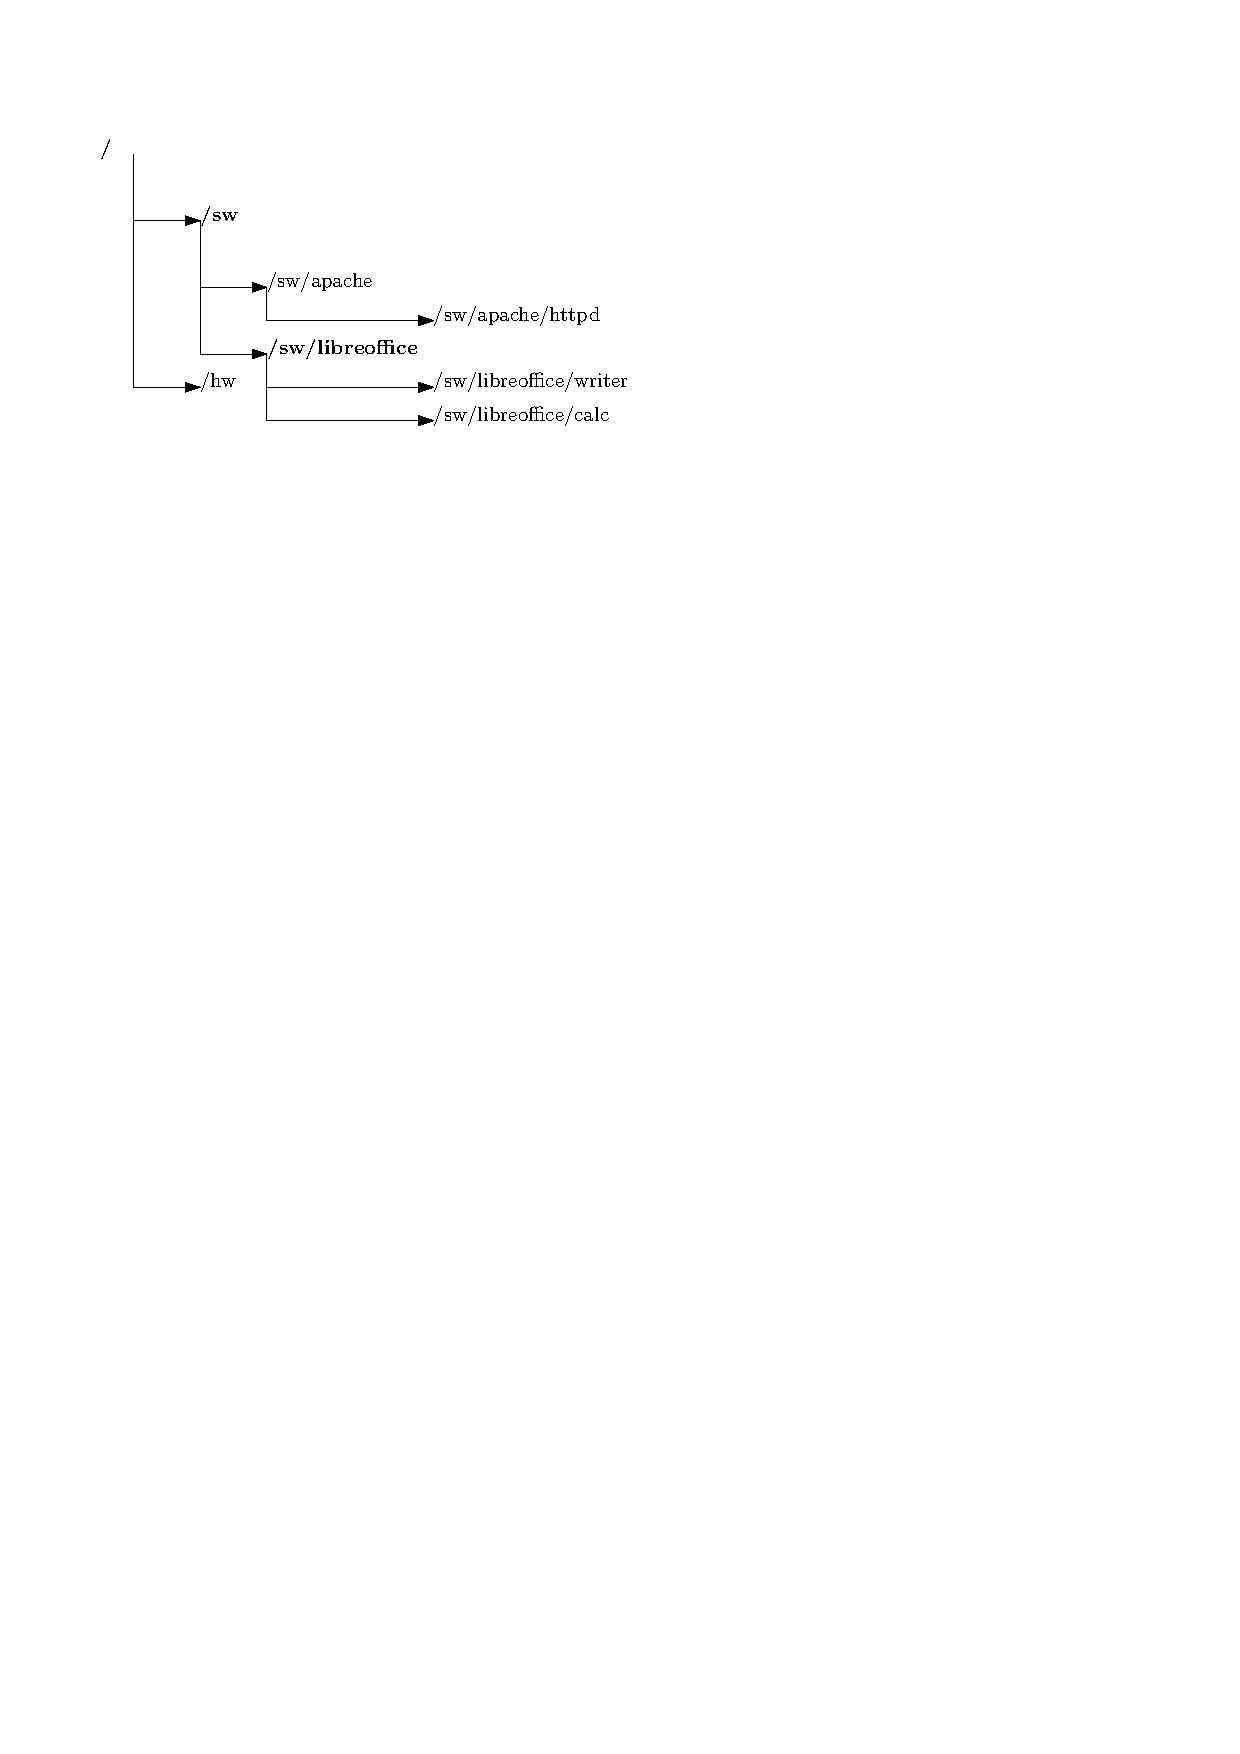
\includegraphics{mounting}
\end{frame}

\begin{frame}
	\frametitle{Plugins}

	Different backends can use different plugins:
	\begin{description}[labelsep=10cm,align=right]
	\item[\texttt{/sw}] in the INI file config.ini
	\item[\texttt{/sw/libreoffice}] in the XML file libreoffice.xml
	\end{description}

	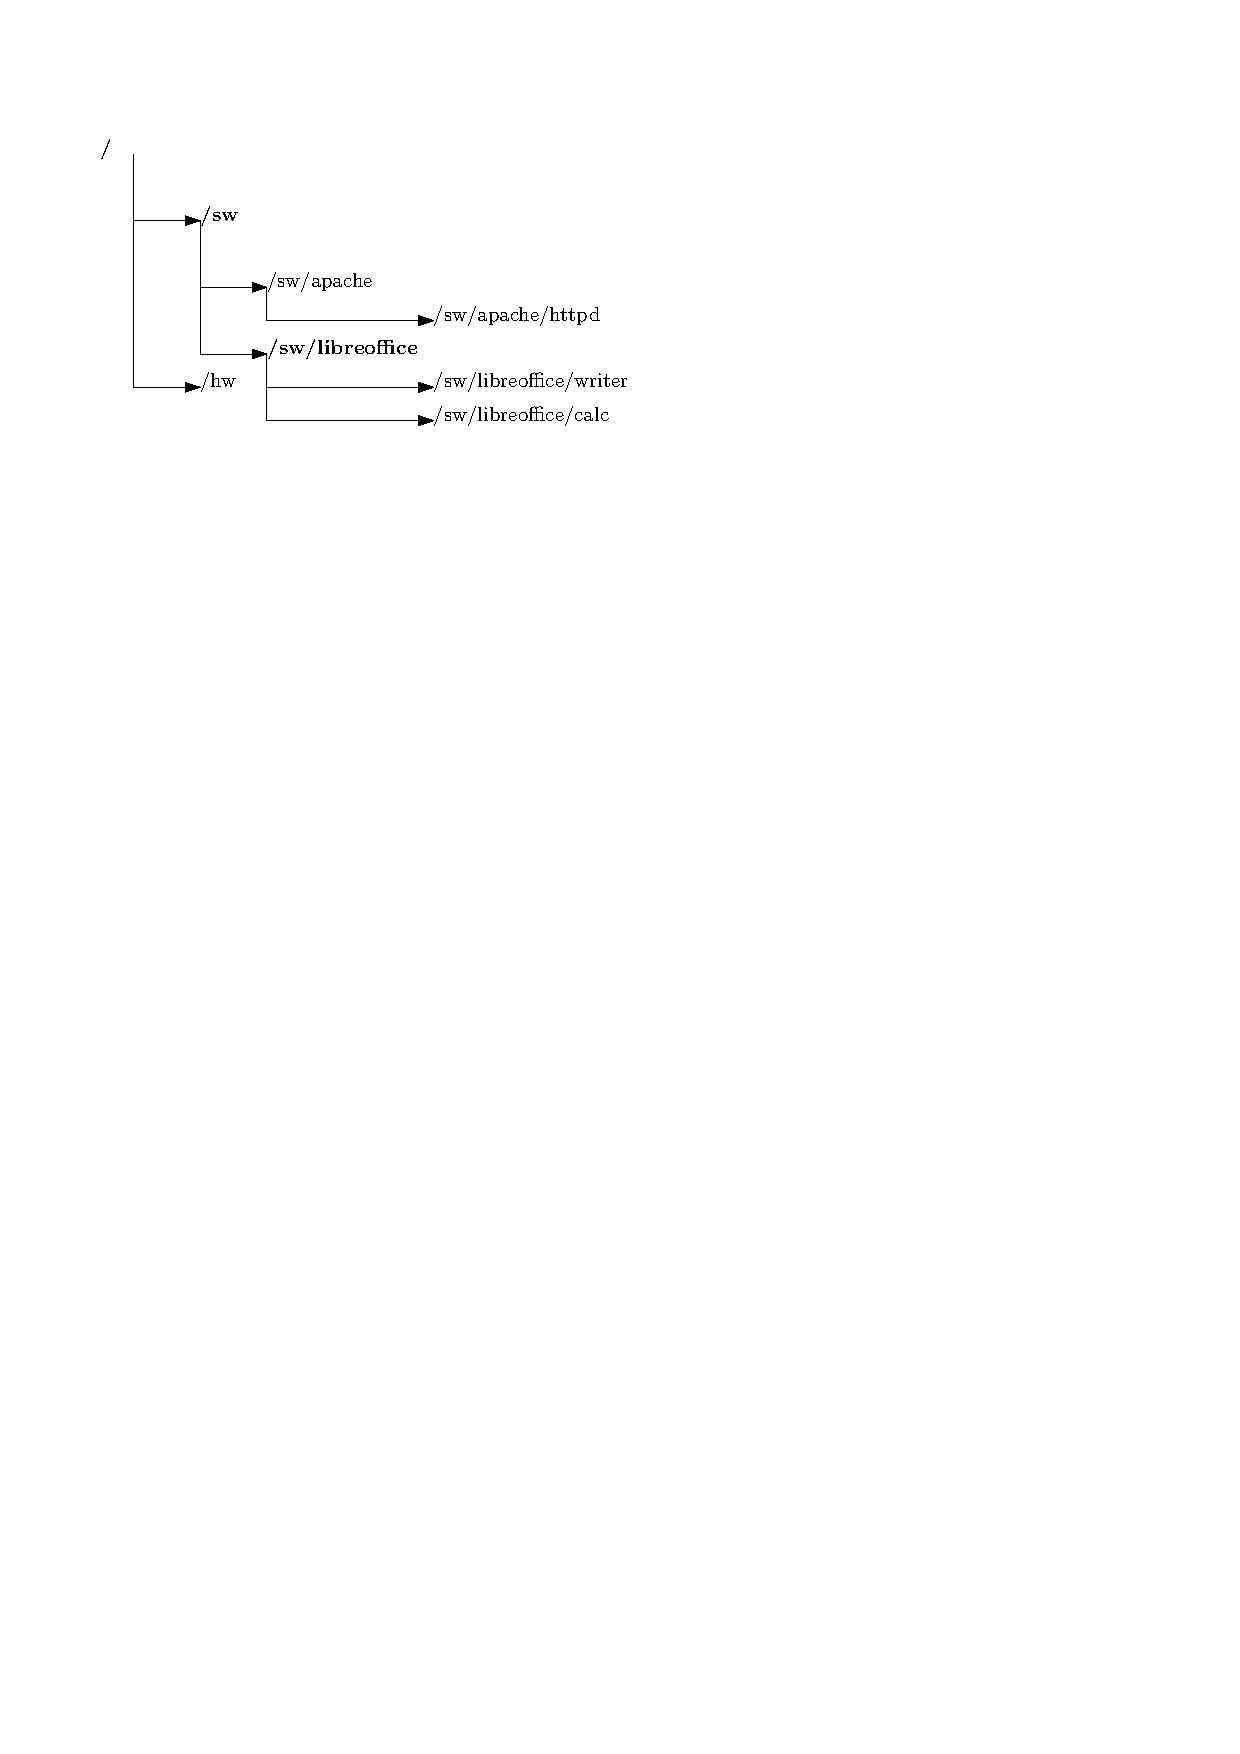
\includegraphics{mounting}
\end{frame}

\begin{assignment}
	\begin{task}
	Explain your neighbor what mounting is.
	\end{task}
\end{assignment}


\subsection{Trend and Outlook}

\begin{frame}
	\frametitle{Trend Firefox}
	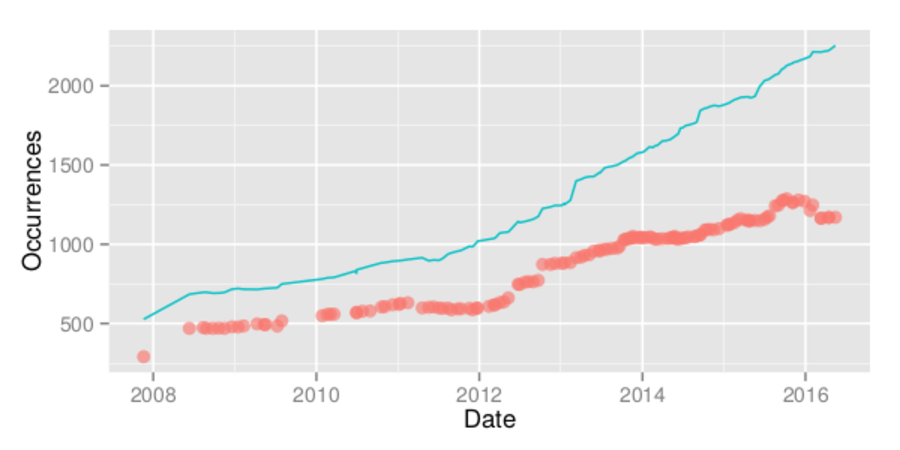
\includegraphics[scale=0.7]{firefox}
\end{frame}

\begin{frame}
	\frametitle{Trend Chromium}
	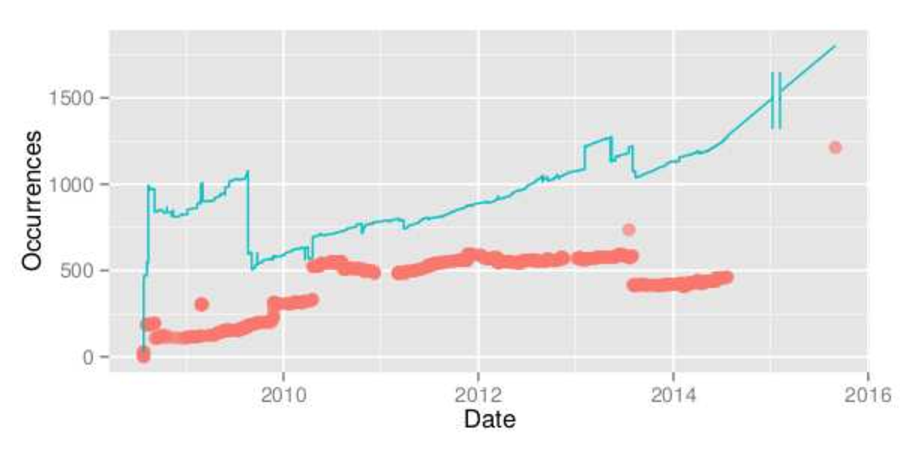
\includegraphics[scale=0.7]{chromium}
\end{frame}

\begin{frame}
	\frametitle{Outlook}
	\begin{itemize}
	\item Environment Variables
	\item Command-line options
	\item Complexity
	\end{itemize}
\end{frame}





\appendix

\begin{frame}[allowframebreaks]
	\bibliographystyle{plainnat}
	\bibliography{../shared/elektra.bib}
\end{frame}

\end{document}

